\documentclass{article}
%
%
%       i_to_the_i_is_real.tex
%
%	David Meyer
%	dmm613@gmail.com
%	15 July 2022
%
%
%   get various packages
%
\usepackage[margin=1.0in]{geometry}                                     % adjust margins
\geometry{letterpaper}                                                  % or a4paper or a5paper or ... 
\usepackage{url}                                                        % need this to use URLs in bibtex
\usepackage{setspace}                                                   % need this for \setstrech{...}
\usepackage{scrextend}                                                  % need this for addmargin
\usepackage[export]{adjustbox}                                          % need this to get frame for includegraphics
%
%   tikz et al
%
\usepackage{tikz}
\usetikzlibrary{calc,patterns,angles,quotes,shapes,math,decorations,
                through,intersections,lindenmayersystems,backgrounds}
\usepackage{circuitikz}                                                 % draw circuits    
\usepackage{pgfplots}
\usepackage{pgfplots}	
%
%	more math stuff
%
\usepackage{amsmath,amsfonts,amssymb,amsthm}
\usepackage{mathtools}
\usepackage{commath}                                                    % get \norm{x}
\usepackage{fixmath}                                                    % get \mathbold
\usepackage{gensymb}                                                    % get \degree
\usepackage{mathrsfs}
\usepackage{hyperref}
\usepackage{subcaption}
\usepackage{authblk}
\usepackage{graphicx}
\usepackage{hyperref}
\usepackage{alltt}
\usepackage{color}
\usepackage{float}
\usepackage{braket}
\usepackage{siunitx}
\usepackage{relsize}
\usepackage{multirow}
\usepackage{esvect}
%
%	watermarks
%
% \usepackage{draftwatermark}
% \SetWatermarkText{Draft}
% \SetWatermarkScale{5}
% \SetWatermarkLightness {0.9} 
% \SetWatermarkColor[rgb]{0.7,0,0}
%
%
%	theorems, definitions, etc
%
\theoremstyle{definition}
\newtheorem{theorem}{Theorem}[section]
\newtheorem{definition}{Definition}[section]
\newtheorem{proposition}{Proposition}[section]
\newtheorem{lemma}{Lemma}[section]
\newtheorem{example}{Example}[section]
\newtheorem{remark}{Remark}[section]
%
%	The following code allows you to do
%
%	\begin{bmatrix}[r] (or [c] or [l])
%
\makeatletter
\renewcommand*\env@matrix[1][c]{\hskip -\arraycolsep
  \let\@ifnextchar\new@ifnextchar
  \array{*\c@MaxMatrixCols #1}}
\makeatother
%
%	make \arg{min,max}_{n \to \infty} work nicely
%
\newcommand{\argmax}{\operatornamewithlimits{argmax}}
\newcommand{\argmin}{\operatornamewithlimits{argmin}}
%
%	handy commands
%
\newcommand*{\Scale}[2][4]{\scalebox{#1}{$#2$}}
\DeclareMathOperator{\E}{\mathbb{E}}
\DeclareMathOperator{\bda}{\Big \downarrow}						% big down arrow
\newcommand{\veq}{\mathrel{\rotatebox{90}{$=$}}}

%
%	Title, author and date
%
\title{Why is $i^i$ a real number?}
\author{David Meyer \\ \href{mailto:dmm613@gmail.com}
                            {dmm613@gmail.com}}
\date{Last update: \today}
%
%
%
\begin{document}
\maketitle
%
%
%
\section{Introduction}
There are a many ways to think about this somewhat perplexing
question. But first we look at why a complex number $z$ equals
$r\mathrm{e}^{i \theta}$. Then in Section \ref{sec:automorphism}
we use the fact that complex conjugation is an automorphism of
$\mathbb{C}$ to show that $i^i \in \mathbb{R}$.  In Section
\ref{sec:power_series} we use the power series expansion of $i^i$
to show that $i^i \in \mathbb{R}$, and in Section
\ref{sec:eulers_formula} we rely on Euler's formula to show the
same result. In Section \ref{what_does_i_to_the_i_equal} we do a
bit of arithmetic to show the numerical value of $i^i$. Finally
Section \ref{sec:conclusions} offers a few conclusions.

\bigskip
\noindent
Before launching into all of this, note that we will make heavy
use of the exponential function $\exp(z)$ (and therefore as you
might expect, this means heavy use of $\log(z)$. The important
point for this discussion is that $\exp(z)$ is injective over
$\mathbb{R}$ but not over $\mathbb{C}$. More specifically, for a
complex number $z$ the the complex logarithm $\log(z)$ is defined
as the inverse function to the exponential function. That is, it
satisfies $e^{\log z} \equiv z$. Now since $re^{i\theta} =
re^{i(\theta+2k\pi)}$ for all $k \in \mathbb{Z}$ we have that for
any choice of $k$, $\log(re^{i(\theta+2k\pi)})$ is a valid
inverse for $re^{i\theta}$. The logarithm is therefore a
multivalued function and each value of $k$ defines what is called
a different \emph{branch} of the logarithm. The \emph{principal branch}
usually refers to the choice $k=0$ \cite{wiki:principle_branch}. 
See Remark \ref{remark:complex_logarithm} for a bit more on this point.


\bigskip
\noindent
One note here: I will use "log" to denote the natural log ($\log_{e}$) 
of the principal value of the logarithm of $z$, noting that some 
authors "Log" to distinguish the principal value from other logarithms 
of $z$ \cite{wiki:complex_logarithm}. 
%
%
%
\section{First: A Bit of Review}
\label{sec:why_is_z_equal_r}
This section reviews the nature of a complex number $z$, where
the length of the line from the origin to the point $z$, $|z|$,
equals $r$. In particular, why does a complex number $z = r 
\mathrm{e}^{i \theta}$? To see why this is the case, first 
consider the complex plane, shown in Figure \ref{fig:complex_plane}:

\medskip
\begin{figure}[H]
\centering
  \resizebox{0.35 \textwidth}{!} {														% resize figure if you want
    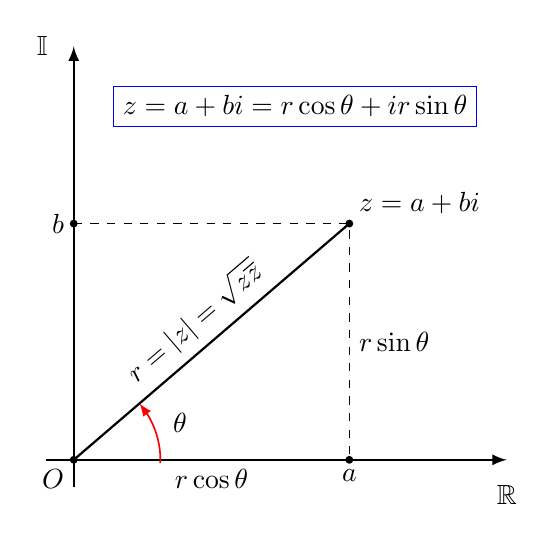
\begin{tikzpicture} [every edge quotes/.append style = {anchor=south, sloped}]		%
		\coordinate (O) at (0,0);                                                       % name a coordinate for the origin
%
%	draw axes, saving the real part to calculate the angle (below)
%
		\draw[thick, -latex] (-0.35,0.00) -- (5.50,0.00) coordinate[yshift=-0.20cm,label=below: $\mathbb{R}$] (x);
		\draw[thick, -latex] (0.00,-0.35) -- (0.00,5.25) node[xshift=-0.2cm,left] {$\mathbb{I}$}
				node[draw,rectangle,thin,blue,below right=5.0mm]						%
            		{$\color{black}{													%
						z = a + bi =													% z = <a bunch of stuff>
						r \cos \theta + i r \sin \theta}$};								%
		\coordinate[label=below left:$O$] (O);                                          % label origin
		\fill (O) circle(0.05);                                                         % draw a black dot at the origin
		\fill (3.5,3) coordinate[label=above right:{$z = a + bi $}] (z) circle(0.05);   % draw phasor and a dot (circle(0.05))
		\draw[dashed] (0,3) node[left] {$b$} -| (3.5,0) node[below] {$a$};              % draw dashed lines to a and b
		\draw [draw=none] (0,0) -- (3.5,0) node [midway, below]{${r \cos \theta}$};     % use [draw=none] to put label midway
		\draw [draw=none] (3.5,3.0) -- (3.5,0) node [midway, right]{${r \sin \theta}$};	% use [draw=none] to put label midway
		\fill (0,3) circle(0.05);                                                       % draw a dot on the y axis at b 
		\fill (3.5,0) circle(0.05);                                                     % draw a dot on the y axis at a
		\draw[thick] (O) to ["$r = |z|=\sqrt{z\overline{z}}$"] (3.5,3);                 % label r
		\pic [draw=red, line width=0.60pt, -latex , angle radius=11mm,                  % draw the angle, making the arc a bit thicker
				angle eccentricity=1.3, "$\theta$"] {angle = x--O--z};          		% calculate the angle theta
     \end{tikzpicture}																	% end tikzpicture
  }																						% end resizebox
 \caption{The Complex Plane}
 \label{fig:complex_plane}
\end{figure}

\smallskip
\noindent
Figures \ref{fig:complex_plane} and \ref{fig:eulers_formula} give us a pretty 
way to see why $z = r \mathrm{e}^{i\theta}$:
\begin{equation*}
\begin{array}{lllll}
z
&=& a + ib
                &\hspace{6em} \mathrel{\#} \text{definition of a point $z$ in the complex plane} \\ 
[2pt]
&=&  r \cos \theta + i r \sin \theta
                &\hspace{6em}\mathrel{\#} \text{switch to polar coordinates: $a = r \cos
				\theta$ and $b = r \sin \theta$} \\ 
[2pt]
&=&  r \left ( \cos \theta +i \sin \theta \right )
                &\hspace{6em}\mathrel{\#} \text{factor out  $r$} \\ 
[2pt]
&=& r \mathrm{e}^{i\theta}
                &\hspace{6em}\mathrel{\#}\text{$e^{i\theta} = \cos \theta + i \sin \theta$
				(Euler's formula \cite{wiki:eulers_formula})} 
\end{array}
\end{equation*}

\noindent
So we see that $z = r \mathrm{e}^{i\theta}$. $\blacksquare$
%
% Euler's formula on the unit circle in the complex plane
%
\begin{figure}[t]
\centering
  \resizebox{0.42 \textwidth}{!} {                                                     % resize figure if you want
    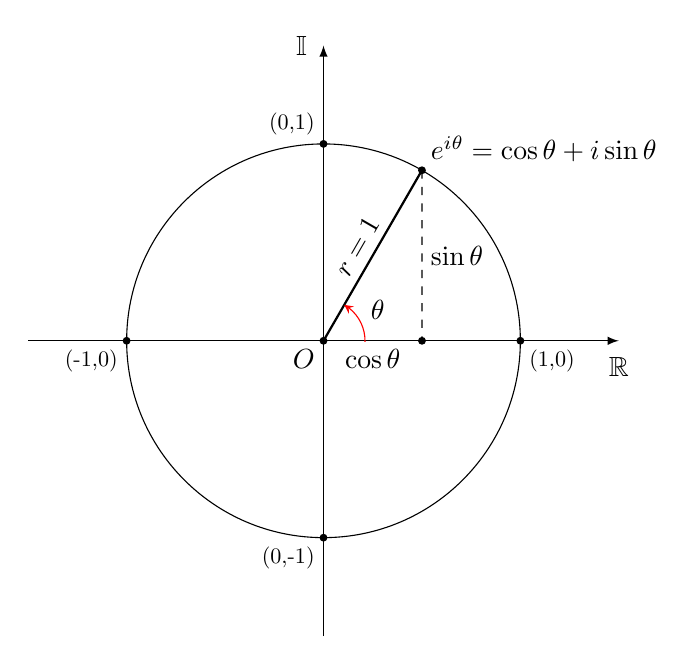
\begin{tikzpicture}[>=stealth, inner sep=3pt,scale=2.5]
      \draw[-latex] (-1.5,0) -- node[below left]{$O$} (1.5,0)
                coordinate[yshift=-0.10cm,label=below:$\mathbb{R}$](x);                 % make and label the axes
      \fill[black] (0,0) circle(0.02);                                                  % draw a black dot at the origin
      \draw[-latex] (0,-1.5) -- (0,1.5) node[xshift=-0.10cm, left]{$\mathbb{I}$};
      \draw (0,0) coordinate(o) circle [radius=1cm];                                    % draw unit circle
      \coordinate (p) at (60:1);                                                        % 60 degrees with r = 1
      \fill (p) coordinate[label={above right: ${e^{i\theta} =
                \cos \theta + i \sin \theta}$}] (p) circle(0.02);                       % Euler's formula 
      \coordinate (q) at (p|-o);
%
% draw the various 1s around the unit circle
%
     \coordinate (a) at (0,1);
     \fill (a) coordinate [label={above left: ${\scalebox {0.80}
                          {(0,1)}} $}] (a) circle(0.02);                                % draw coordinates (making them a bit smaller) 
     \coordinate (b) at (-1,0);
     \fill (b) coordinate [label={below left:${\scalebox {0.80}
                          {(-1,0)}}$}] (b) circle(0.02);                                % draw coordinates
     \coordinate (c) at (0,-1);
     \fill (c) coordinate [label={below left:${\scalebox {0.80}
                          {(0,-1)}}$}] (c) circle(0.02);                                % draw coordinates
     \coordinate (d) at (1,0);
     \fill (d) coordinate [label={below right:${\scalebox {0.80}
                          {(1,0)}}$}] (d) circle(0.02);                                 % draw coordinates
%
%       do the rest of the labeling and draw the angle
%
     \draw[thick,line join=round] (o) -- node[rotate=60,above]{$r = 1$}(p);             % label r
     \draw [dashed] (p) -- (q) node [midway, right]{${\sin \theta}$}; 
     \draw [] (q) -- (o) node [midway, below] {${\cos \theta}$};        
     \fill (q) coordinate [] (q) circle(0.02);                                          % put a dot at (q)
     \pic[draw=red,"$\theta$",angle radius=15pt,angle
                   eccentricity=1.5,->]{angle=x--o--p};                                 % draw the angle 
    \end{tikzpicture}                                                                   % end tikzpicture
  }                                                                                     % end resizebox
\caption{Euler's Formula, the Unit Circle, and the Complex Plane}
\label{fig:eulers_formula}
\end{figure}
%
%
%
\section{Automorphism of $\mathbb{C}$}
\label{sec:automorphism}
In this section we look at solving this puzzle using the fact
that complex conjugation is an automorphism of $\mathbb{C}$
\cite{complex_conjugation_is_automorphism}. For this approach we
need the following facts:

\begin{enumerate}
\item If a complex number $z$ equals its complex
conjugate $\overline{z}$ then $z \in \mathbb{R}$
\label{item:complex_conjugate}

\item $-i = i^{-1}$
\label{item:minus_i}

\item $\overline{z} = r \mathrm{e}^{-i\theta}$
\label{item:overline_z}
\end{enumerate}


\noindent
To see \ref{item:complex_conjugate}., consider the following
argument: Let $z$ be a complex number so that $z = a+bi$. Then
$\overline{z} = a-bi$. So $z = \overline{z} \Rightarrow a+bi =
a-bi$. Subtracting $a$ from both sides of the right hand side of
this implication gives us $bi = -bi$ or $2bi = 0$. Since we know
that $2 \neq 0$ and $i \neq 0$ it must be the case that
$b=0$. Said another way: $\operatorname{Im}(z) = 0$ and
$\operatorname{Re}(z) = z$. That is, $z \in \mathbb{R}$. So if $z
= \overline{z}$ we know that $z \in \mathbb{R}$.

\bigskip
\noindent
To see \ref{item:minus_i}., notice that $-(i\cdot i) = -i^2 =
-(-1) = 1$ and $-i \cdot i = 1 \Rightarrow -i = i^{-1}$.

\bigskip
\noindent
To see \ref{item:overline_z}., consider that for $r,\theta \in \mathbb{R}$ 
we have

\begin{equation*}
\begin{array}{llll}
\overline{z}
&=& \overline{r \cdot (\cos \theta + i \sin \theta)} 
		&\hspace{5em} \mathrel{\#} \text{since $z = r \cdot (\cos\theta+i\sin\theta)$ 
		(Figure \ref{fig:complex_plane})}\\
[5pt]
&=& \overline{r} \cdot \overline{(\cos \theta + i \sin \theta)} 
		&\hspace{5em} \mathrel{\#} \text{since $\overline{z_1 \cdot z_2} = \overline{z_1}\cdot \overline{z_2}$ 
		(product rule for complex conjugation \cite{product_complex_conjugates})} \\
[5pt]
&=& r \cdot \overline{(\cos \theta + i \sin \theta)} 
		&\hspace{5em} \mathrel{\#} \text{since $\overline{r} = \overline{r + 0i} = r - 0i = r$ 
		($\overline{x} = x$ for $x \in \mathbb{R}$)} \\
[5pt]
&=& r \cdot (\cos \theta - i \sin \theta)
		&\hspace{5em} \mathrel{\#} \text{since $\overline{a+bi} = a-bi$} \\
[5pt]
&=& r \mathrm{e}^{-i\theta}
		&\hspace{5em} \mathrel{\#} \text{since $e^{-i\theta} = \cos \theta - i \sin \theta$
		(corollary to Euler's formula \cite{eulers_formula_corollary})}
\end{array}
\end{equation*}

\noindent
Now we want to show that $\overline{i^i} = i^i$, which would
show that $i^i \in \mathbb{R}$ by the above argument\footnote{See 
Remark \ref{remark:complex_logarithm} for a bit on what is still
open here.}. So consider

\begin{equation*}
\begin{array}{llll}
\overline{i^i}
&=& {\overline{i}}^{\overline{i}}       &\hspace{13em} \mathrel{\#} \text{see proof below} \\
[5pt]
&=& (-i)^{-i}                           &\hspace{13em} \mathrel{\#} \text{since $i = 0+1i$ and $\overline{0+1i} = -1i = -i$} \\
[5pt]
&=& {(i^{-1})}^{-i}                     &\hspace{13em} \mathrel{\#} \text{since $-i = i^{-1}$ (item \ref{item:minus_i}. above)} \\
[5pt]
&=& i^{(-1 \cdot -i)}                   &\hspace{13em} \mathrel{\#} \text{since ${(x^m)}^{n} = x^{mn}$} \\
[5pt]
&=& i^i                                 &\hspace{13em} \mathrel{\#} \text{since $-1 \cdot -i = i$}
\end{array}
\end{equation*}

\medskip
\noindent
So we see that $\overline{i^i} = i^i$, which implies that $i^i \in
\mathbb{R}$. $\blacksquare$ 

\bigskip
\noindent
This is all good, but why does $\overline{i^i} = {\overline{i}}^{\overline{i}}$?
To see why first notice that

\medskip
\begin{equation*}
\begin{array}{llll}
\log (\overline{z})
&=& \log(r \mathrm{e}^{-i\theta})
		&\hspace{7em} \mathrel{\#} \text{since $\overline{z} = re^{-i\theta}$ (item \ref{item:overline_z}. above)} \\
[5pt]
&=& \log \left (\dfrac{r}{e^{i\theta}} \right) 	
		&\hspace{7em} \mathrel{\#} \text{since $a^{-b} = \dfrac{1}{a^b}$} \\
[12pt]
&=& \log(r) - \log(e^{i\theta})
		&\hspace{7em} \mathrel{\#} \text{by the quotient rule for logarithms \cite{properties_of_logarithms}} \\
[12pt]
&=& \log(r) - i\theta
		&\hspace{7em} \mathrel{\#} \text{since $\log({e^{i\theta}}) = i\theta$} \\
[12pt]
&=& \log(r) + \overline{i\theta}
		&\hspace{7em} \mathrel{\#} \text{since $-i\theta = \overline{0+i\theta} = \overline{i\theta}$} \\
[12pt]
&=& \log(r) + \overline{\log(e^{i\theta})}
		&\hspace{7em} \mathrel{\#} \text{since $i\theta = \log(e^{i\theta})$} \\
[12pt]
&=& \overline{\log(r)} + \overline{\log(e^{i\theta})}
		&\hspace{7em} \mathrel{\#} \text{since $x = \overline{x}$ for $x \in \mathbb{R}$ 
		and $\log(r) \in \mathbb{R}$} \\
[12pt]
&=& \overline{\log(r) + \log(e^{i\theta})}
		&\hspace{7em} \mathrel{\#} \text{by the sum rule for conjugates \cite{sum_of_conjugates}} \\
[12pt]
&=& \overline{\log(re^{i\theta})}
		&\hspace{7em} \mathrel{\#} \text{by the product rule for logarithms \cite{properties_of_logarithms}} \\
[12pt]
&=& \overline{\log(z)} 
		&\hspace{7em} \mathrel{\#} \text{since $z = re^{i\theta}$}	
\end{array}
\end{equation*}

% \begin{equation*}
% \begin{array}{llll}
% \overline{\log(z)}
% &=& \overline{\log(re^{i\theta})}
%                &\hspace{6em} \mathrel{\#} \text{since $z = re^{i\theta}$} \\
% [6pt]
% &=& \overline{\log(r) + \log(e^{i\theta})}
%                 &\hspace{6em} \mathrel{\#} \text{by the product rule for logarithms} \\
% [6pt]
% &=& \overline{\log(r)} + \overline{\log(e^{i\theta})}
%                 &\hspace{6em} \mathrel{\#} \text{by the sum rule for conjugates \cite{sum_of_conjugates}} \\
% [6pt]
% &=& \log(r) + \overline{\log(e^{i\theta})}
%                 &\hspace{6em} \mathrel{\#} \text{since $\log(r) \in\mathbb{R}$} \\
% [6pt]
% &=& \log(r) + \overline{i\theta}
%                 &\hspace{6em} \mathrel{\#} \text{since $\log (e^{i\theta}) = i\theta$} \\
% [6pt]
% &=& \log(r) - i\theta
%                 &\hspace{6em} \mathrel{\#} \text{since $\overline{i\theta} = \overline{0+i\theta} = -i\theta$} \\
% [6pt]
% &=& \log(r) - \log (e^{i\theta})
%                 &\hspace{6em} \mathrel{\#} \text{since $i \theta = \log (e^{i\theta})$} \\
% [6pt]
% &=& \log (\overline{z})
%                 &\hspace{6em} \mathrel{\#} \text{since $\log (\overline{z}) = \log(r) - \log(e^{i\theta})$}
% \end{array}
% \end{equation*}

\bigskip
\noindent
Note that @antoinechambertloir@mathstodon.xyz says that $\log (\overline{z})$ not necessarily equal
to $\overline{\log(z)}$ (see Remark \ref{remark:complex_logarithm}). However, if it were to be 
correct, then

\smallskip
\begin{equation*}
\begin{array}{llll}
\log(\overline{z^w})
&=& \overline{\log(z^w)}                        &\hspace{9em} \mathrel{\#} \text{this is the result that is in question} \\
[8pt]
&=& \overline{w  \cdot \log(z)}					&\hspace{9em} \mathrel{\#} \text{by the power rule for logarithms} \\
[8pt]
&=& \overline{w} \cdot \overline{\log(z)}       &\hspace{9em} \mathrel{\#} \text{by the product rule for conjugation} \\
[8pt]
&=& \overline{w} \cdot \log(\overline{z})       &\hspace{9em} \mathrel{\#} \text{since $\log (\overline{z}) 
												= \overline{\log(z)}$} \\
[8pt]
&=& \log(\overline{z}^{\overline{w}})           &\hspace{9em} \mathrel{\#} \text{by the power rule for 
												logarithms \cite{properties_of_logarithms}}
\end{array}
\end{equation*}

\bigskip
{\setstretch{1.5}
\noindent
Since $\log(\overline{z^w}) = \log(\overline{z}^{\overline{w})}$ we know that 
$e^{\log(\overline{z^w})} = e^{\log(\overline{z}^{\overline{w}})}$ which in turn 
implies that $\overline{z^w} = \overline{z}^{\overline{w}}$. Setting $z=w=i$ we 
see that $\overline{i^i} = {\overline{i}}^{\overline{i}}$. $\blacksquare$
\par}
\bigskip


\section{Power Series}
\label{sec:power_series}

{\setstretch{1.65} We know that the Taylor series
\cite{wiki:taylor} for $e^x = \sum\limits_{k=0}^{\infty}
\dfrac{x^k}{k!}$.  We also know from Euler's formula
\cite{notes:eulers_formula} that $i = e^{i \frac{\pi}{2}}$ (since
$e^{i\frac{\pi}{2}} = \cos \frac{\pi}{2} + i \sin \frac{\pi}{2} =
i$).  Note that the same result can be obtained with $x \in \left
\{\frac{\pi}{2}, \frac{5 \pi}{2}, \frac{9\pi}{2}, \hdots \right
\}$, so in general $x = \frac{\pi}{2} \cdot (1+4n)$ where $n \in
\mathbb{N} \cup \{0\}$.  \par}

\bigskip
\noindent
So we see that

\medskip
\begin{equation*}
\begin{array}{llll}
i^t 
&=& {\big ( e^{\frac{i\pi}{2}} \big )}^t 
		&\hspace{7em} \mathrel{\#} \text{Euler's formula for $i$, 
		raised to the power $t$}\\
[8pt]
&=& e^{\frac{it\pi}{2}}
		&\hspace{7em} \mathrel{\#} \text{since ${(x^m)}^{n} = x^{mn}$} \\
&=& \sum\limits_{k=0}^{\infty} \dfrac{{\big (\frac{it\pi}{2} \big )}^k}{k!}
		&\hspace{7em} \mathrel{\#} \text{since $e^x = \sum\limits_{k=0}^{\infty} \dfrac{x^k}{k!}$ 
		and $x = \frac{it\pi}{2}$} 

\end{array}
\end{equation*}

\bigskip
\noindent
If we let $t = i$ we get $i^i = e^{i^2 \frac{\pi}{2}} =
e^{-\frac{\pi}{2}}$. So $i^i = e^{-\frac{\pi}{2}}$ and since
$e^{-\frac{\pi}{2}} \in \mathbb{R}$ we know that $i^i \in
\mathbb{R}$. Fortunately this agrees with the result we find 
in Section \ref{sec:eulers_formula}. $\blacksquare$


\section{Euler's Formula}
\label{sec:eulers_formula}

\noindent
Another approach is to consider Euler's 
formula evaluated at $x =\frac{\pi}{2}$: 

\smallskip
\begin{equation*}
\begin{array}{lllll}
e^{ix}
&=& \cos x + i \sin x                           	&\hspace{7em} \mathrel{\#} \text{Euler's formula}   \\
[2pt]
&\Rightarrow& e^{i \frac{\pi}{2}} = \cos \frac{\pi}{2} + i \sin \frac{\pi}{2}
                                                	&\hspace{7em} \mathrel{\#} \text{set $x = \frac{\pi}{2}$} \\
[2pt]
&\Rightarrow& e^{i \frac{\pi}{2}} = 0 +  i \cdot 1
                                                	&\hspace{7em} \mathrel{\#} \cos \frac{\pi}{2} = 0
                                                	  \text{ and} \sin \frac{\pi}{2} = 1 \\
[2pt]
&\Rightarrow& e^{i \frac{\pi}{2}}  =  i         	&\hspace{7em}\mathrel{\#} \text{simplify} \\
[2pt]
&\Rightarrow& {(e^{i \frac{\pi}{2}})}^i =  i^i  	&\hspace{7em} \mathrel{\#} \text{raise both sides to $i$} \\
[2pt]
&\Rightarrow& e^{\frac{i^2 \pi}{2}} =  i^i      	&\hspace{7em} \mathrel{\#}  {(x^m)}^n = x^{mn} \\
[2pt]
&\Rightarrow& e^{- \frac {\pi}{2}} =  i^i       	&\hspace{7em} \mathrel{\#} i^2 = -1 \\
[2pt]
&\Rightarrow& e^{- \frac {\pi}{2}} \in \mathbb{R} \Rightarrow i^i \in \mathbb{R}
                                               		&\hspace{7em} \mathrel{\#} \text{$i^i$ is a real number} 
\end{array}
\end{equation*}

\medskip
\noindent
It is important to notice that this expression is multivalued,
and when we evaluate it at $\frac{\pi}{2}$ we are on the
principle branch. However, the same result can be obtained with
$x \in \left \{\frac{\pi}{2}, \frac{5 \pi}{2}, \frac{9\pi}{2},
\hdots \right \}$.  In general $x = \frac{\pi}{2} \cdot (1+4n)$
for $n \in \mathbb{N} \cup \{0\}$. $\blacksquare$


\section{Ok, $i^i \in \mathbb{R}$, but what does it equal}
\label{what_does_i_to_the_i_equal}
We saw above that $i^i = e^{- \frac {\pi}{2}}$. So 
$i^i = e^{- \frac {\pi}{2}} \approx 0.20788$.

\bigskip
\begin{figure}[H]
\center{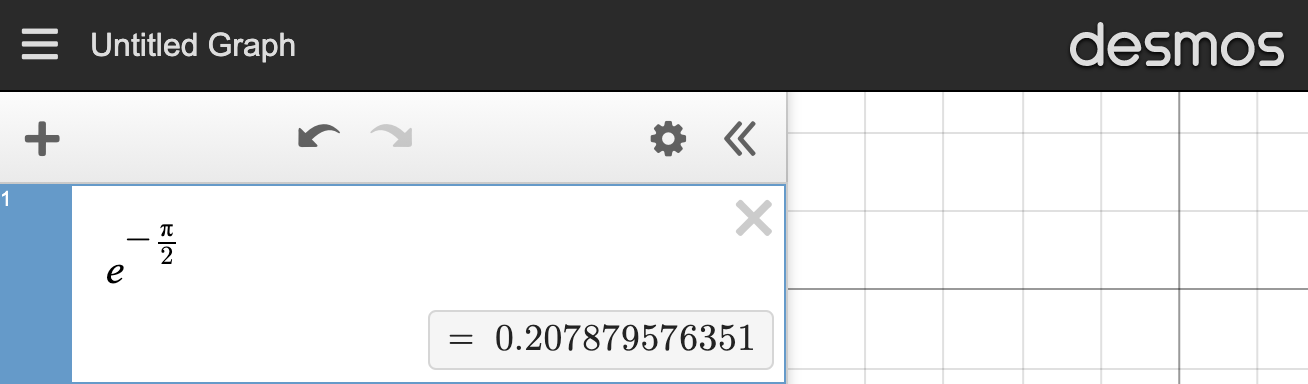
\includegraphics[frame,scale=0.45] {images/e_to_the_minus_pi_over_two.png}}
\end{figure}
%
%
%
\section{Conclusions}
\label{sec:conclusions}
\begin{remark}
\label{remark:complex_logarithm}
Antoine Chambert-Loir (@antoinechambertloir@mathstodon.xyz) tells
me that restricting the logarithm to any particular branch causes
all algebraic relations break down. The example he gives is that
$a^c \times b^c = (ab)^c$ only when the sum of the principal
arguments of $a$ and $b$ equals the principal argument of $ab$
\cite{principal_argument}. Apparently a similar problem arises
for conjugacy when $a$ is strictly negative. I must admit that
I don't fully understand this comment.


\bigskip
\noindent
@antoinechambertloir@mathstodon.xyz also says that "the complex log either is multivalued, 
or requires the a priori choice of a determination of the argument, so that the formula for 
$\log (\overline{z})$ is incorrect: with the choice of principal determination, it is the conjugate 
of $\log(z)$ only when $z$ is not strictly negative. And $\log(-1) = i\pi$ is not its conjugate."
\end{remark}

%
%
%
\smallskip
\section*{Acknowledgements}
Thanks to Dima Pasechnik (@dimpase@mathstodon.xyz), Andrés
E. Caicedo (@AndresCaicedo@mathstodon.xyz), Ben Reiniger
(@bmreiniger@mathstodon.xyz) and Dave Neary (@dneary@mastodon.ie)
for their many helpful comments.
%
%	LaTeX source on overleaf.com
%
\section*{\LaTeX \hspace{0.10 mm} Source}
\url{https://www.overleaf.com/read/cfjttjzdbfnc}
%
%	get a bibliography
%
%	Note:.bib files go in ~/Library/texmf/bibtex/bib with TeXShop (MacTeX).
%	You can also use an absolute path, e.g. \bibliography{/Users/dmm/papers/bib/qc}
%
\bibliographystyle{plain}
\bibliography{qc}
%
%	done
%
\end{document} 


